\newpage
\subsection {Diagramme de séquence}
\subsubsection{Lancement du jeu}
\begin{figure}[H]
    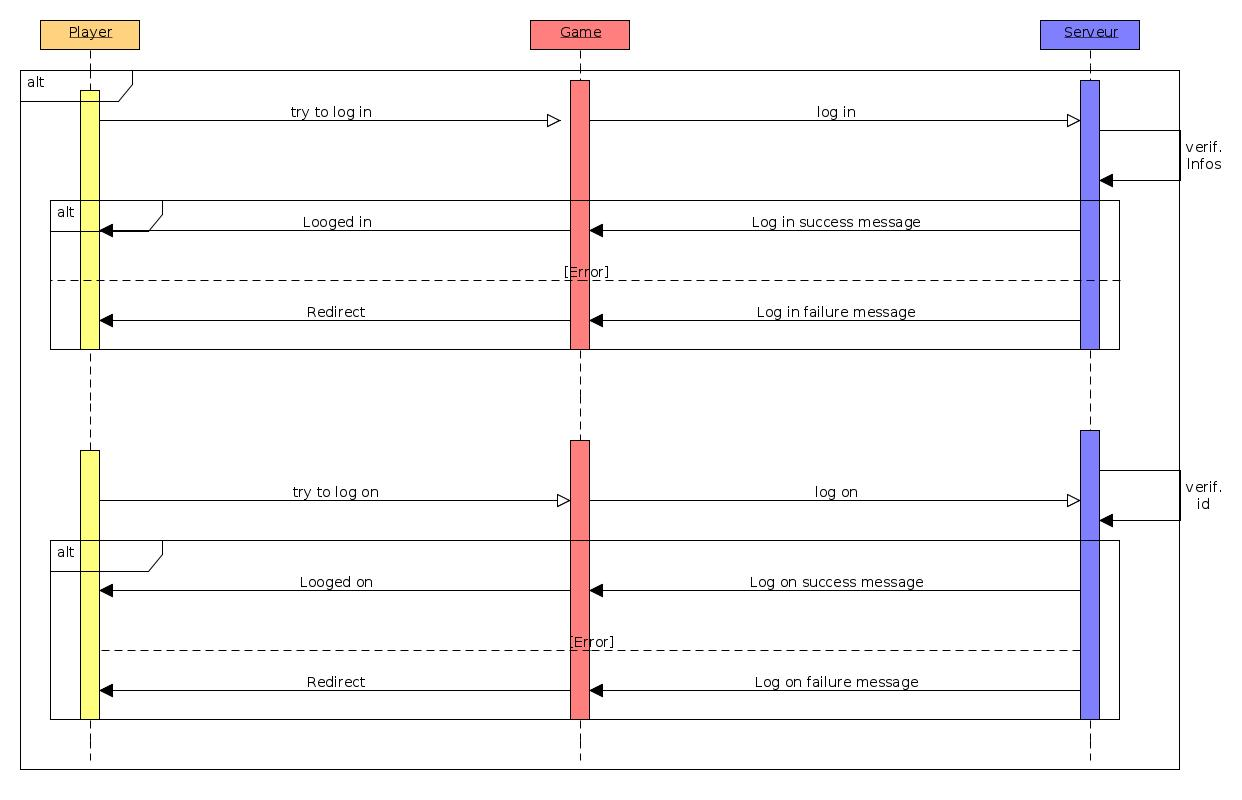
\includegraphics[width=1\textwidth,height=0.9\textwidth]{Images/ConnexionSequanceDiagram.jpg}
    \caption{\label{Connexion Sequence Diagramm} Diagramme de séquence lancement du jeu}
\end{figure}
\noindent\textbf{Analyse}\\
{Ce diagramme a pour but de montrer les différentes alternatives qui peuvent avoir lieues lors du lancement du jeu. Soit l'utilisateur a un \index{account}account et donc il doit se connecter moyennant son identifiant et son mot de passe. Si ces informations sont correctes, alors il sera connecté normalement. Dans le cas contraire il sera redirigé. Soit le joueur ne possède pas de l'\index{account}account et donc doit en créer un. La seule vérification faite ici est l'existence de l'identifiant dans le serveur.
\\Les classes : "Serveur" et "BridgeClass" sont des éventuelles classes à rajouter dans le futur . 
}
\subsubsection{Gestion des événements}
\begin{figure}[H]
    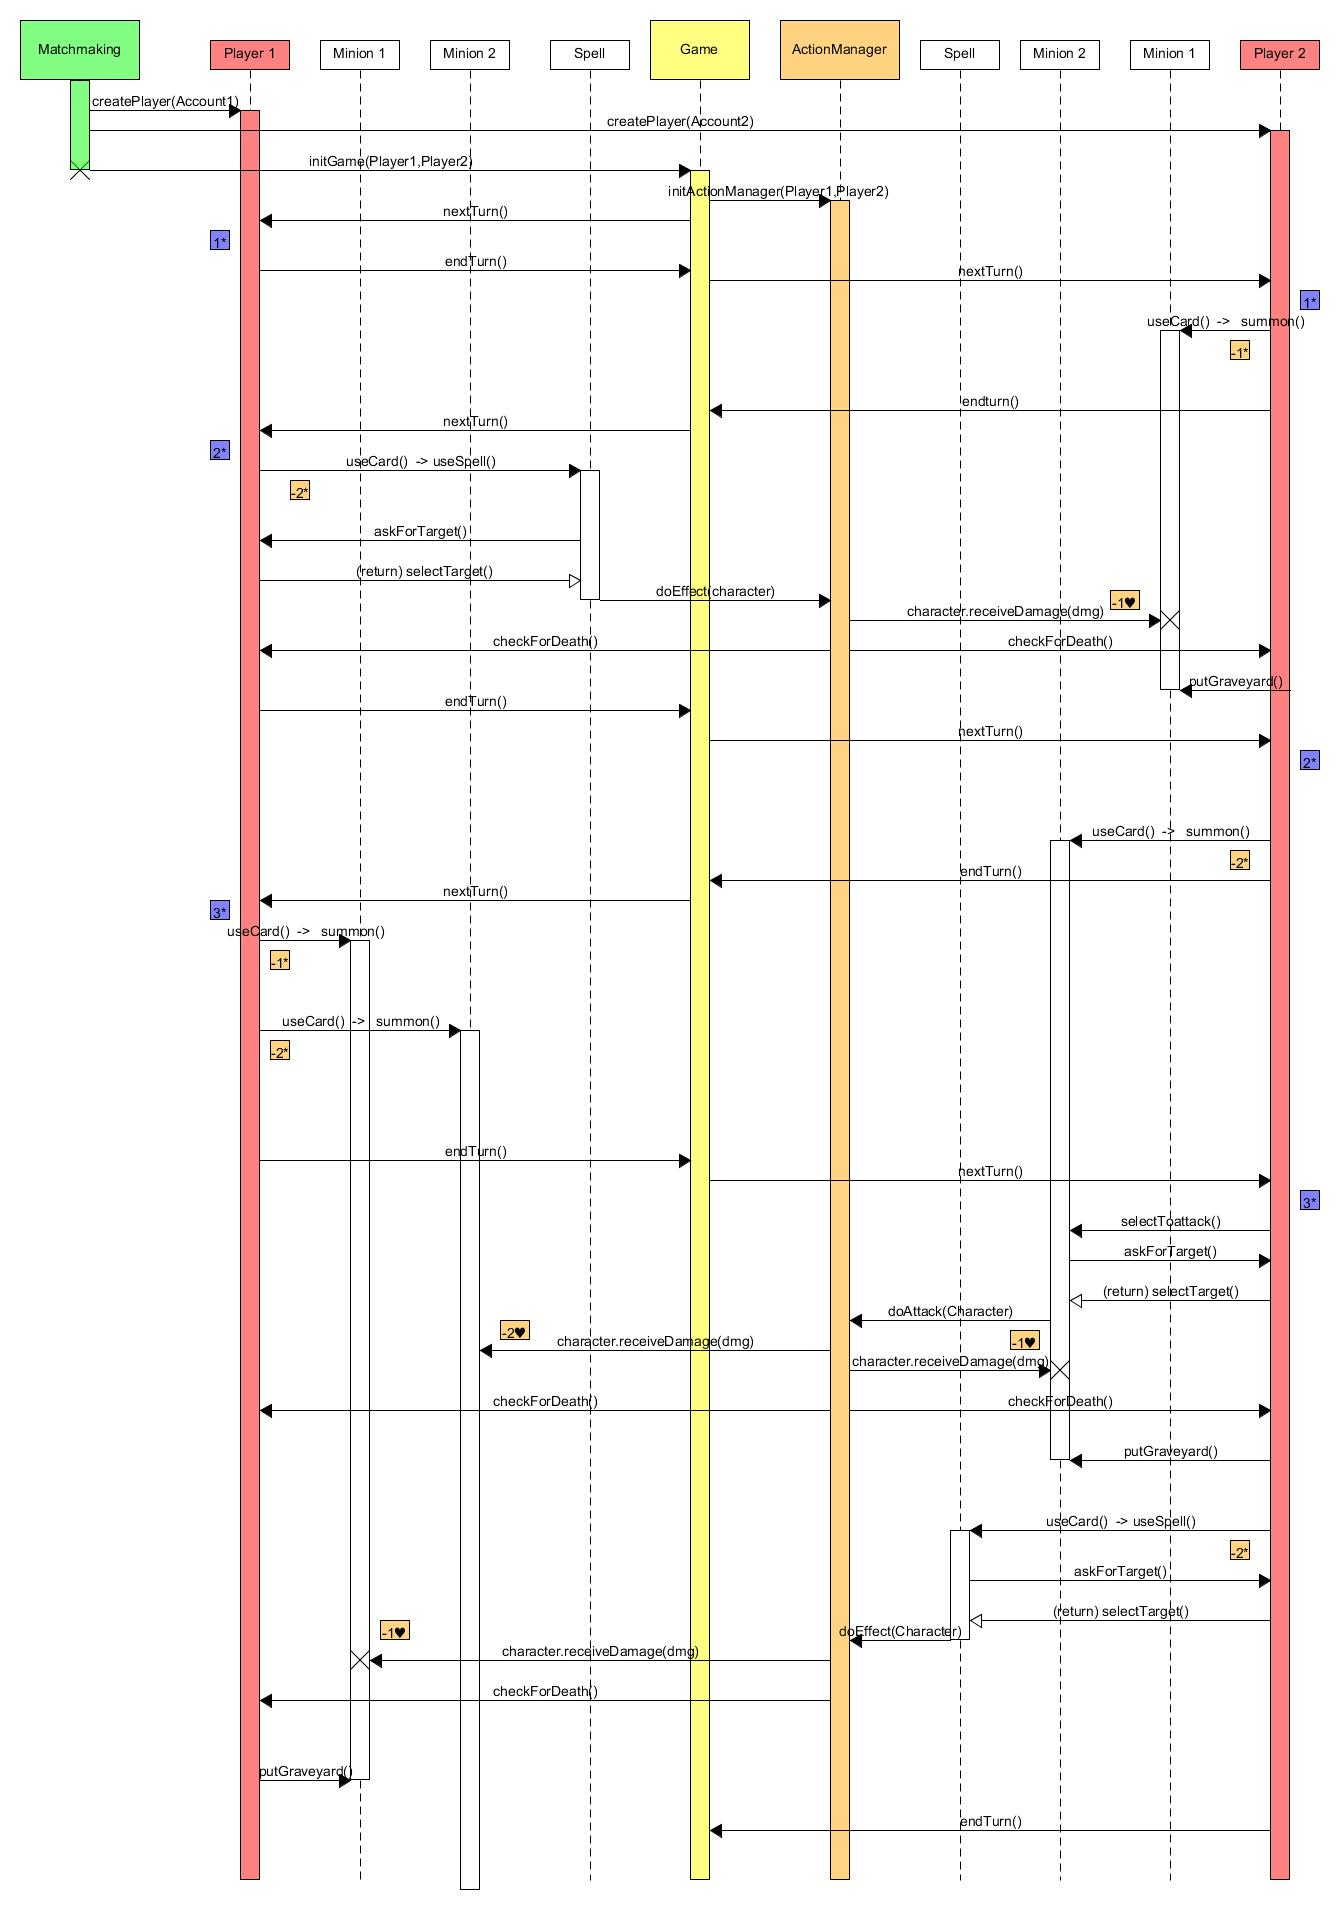
\includegraphics[width=1\textwidth,height=1.35\textwidth]{Images/Sequence-Diagram.jpg}
    \caption{\label{Sequence Diagram Partie} Diagramme de séquence d'un début de partie}
\end{figure}
\noindent\textbf{Analyse}\\
Ce diagramme de séquence a pour but de visualiser les interactions entre certaines classes lors du début d'une partie. Lorsque le \index{Matchmaking} a trouvé deux personnes prêtes à s'affronter, il instancie le Player 1 et le Player 2. Avant d'être détruit, il instanciera également la partie, c'est-à-dire Game, qui, elle, instanciera à son tour l'ActionManager gérant les modifications des objets de type charcater\index{character}. Dans cette section, nous illustrerons seulement le contexte du diagramme ci-dessus. Il ne va sans dire que le déroulement de chaque début de partie est différent.\\
La Game donne la main au Player 1 pour lui signaler que c'est son tour. Comme il n'a qu'un point d'energie et qu'il n'a aucune carte, il ne peut pas jouer et cède son tour.\\
Le Player 2, quant à lui, possède un minion coûtant un point d'energie et décide de l'invoquer.\\
Le Player 1 décide d'utiliser un spell\index{spell} afin de détruire le minion de son adversaire. Le Player 2, voyant son minion détruit, le place ensuite dans son graveyard. Le tour du Player 1 est terminé.\\
À ce stade, le Player 2, n'ayant que deux points d'energie est limité dans ses choix. Il invoque ainsi un autre minion coûtant, cette fois-ci, deux points d'energie.\\
Le Player 1 est en avance d'un point d'energie par rapport au Player 2 puisqu'il a commencé en premier. Il juge nécessaire d'agir comme son adversaire et de rentabiliser ses points et choisit d'invoquer deux minions lors de ce tour-ci.\\
Voyant un certain danger s'approcher, le Player 2 opte pour la minimisation des dégâts et décide de sacrifier son seul minion afin d'abattre le carachter le plus faible de son adversaire. Les deux joueurs placent respectivement leur minion mort dans leur graveyard. Par la suite, le Player 2 lance un spell\index{spell} dans le but d'affaiblir le minion restant de son adversaire.




\subsubsection{Fin de partie}
\begin{figure}[H]
    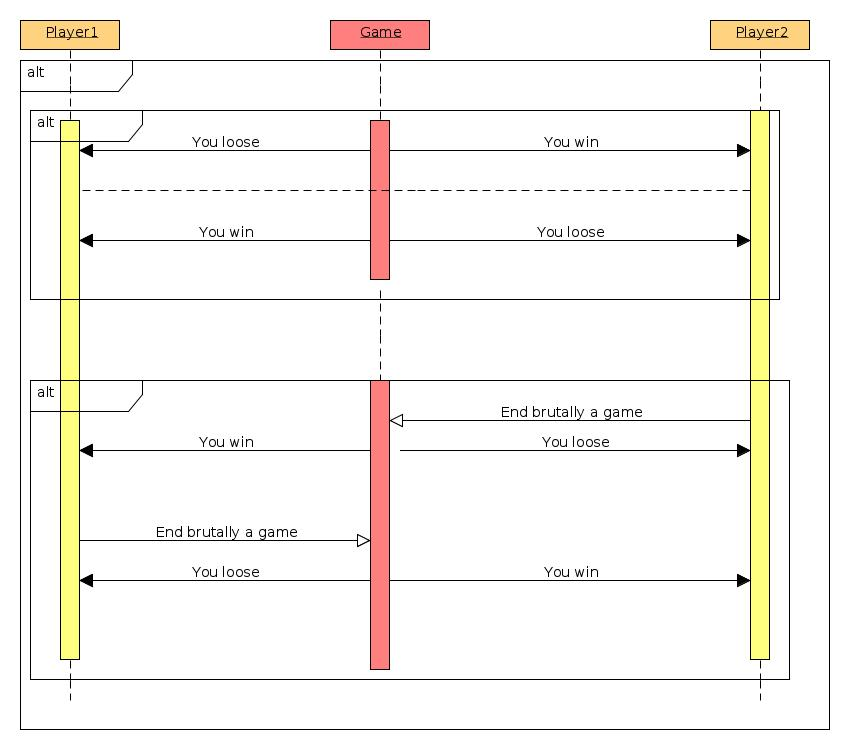
\includegraphics[width=1\textwidth,height=0.9\textwidth]{Images/EndGameSequenceDiagramm.jpg}
    \caption{\label{Endgame Sequence Diagramm} Diagramme de séquence d'une fin de partie}
\end{figure}
\noindent\textbf{Analyse}\\
{Ce diagramme a pour but de montrer les différentes alternatives qui peuvent se dérouler dans une fin de partie , et donc soit un des deux joueurs gagne le match soit l'un des deux quitte la partie et donc la victoire est attribuée à l'adversaire .
}